\section*{7. GPU Mining}
\addcontentsline{toc}{chapter}{GPU Mining}
GPU mining involves the use of a gaming computer’s graphics processing unit to solve complex math problems to verify electronic transactions on a blockchain.\vspace{.3 cm}

Normally, to mine a cryptocurrency, digital coins must be built on a blockchain architecture that supports proof-of-work (PoW) mining. Cryptocurrencies like Bitcoin (BTC), Ethereum (ETH), Monero (XMR), Litecoin (LTC) and Dogecoin (DOGE) are examples of coins that can be mined.\vspace{.3 cm}

\subsection*{7.1 NVIDIA GeForce GTX 1070: The Most Popular Cryptocurrency Mining GPU}
While there are a lot of different graphics cards in the markets, the cards used for crypto mining are those specially designed for gaming, not for video rendering. Shares in GPU manufacturing companies like NVIDIA and AMD have skyrocketed as miners look to earn cryptos with their computing powers. The NVIDIA GeForce GTX 1070 is one of the most popular mining rigs, when considering both its electricity usage, although there are other models out there if you do your own research into will can work for you.\vspace{.3 cm}

While it used to be possible mine Bitcoin and other cryptocurrencies at home with your laptop, that's no longer an option for most cryptos due to the rising interest in mining, along with the Bitcoin reward halvings. Most mining operations, including the use of graphics cards and specialized mining rigs, are now conducted in shared pools, where participants combine their computing powers into a big group to generate results more quickly. Rewards are handed out to miners after a block of the currency has been mined.\vspace{.3 cm}

All the participants in a shared pool get a share in the profits based on how much computing power they contributed. In this way, individual computers represent workers in a mine getting paid for searching for the treasure, the block reward.\vspace{.3 cm}

\begin{figure}[h]
	\centering
	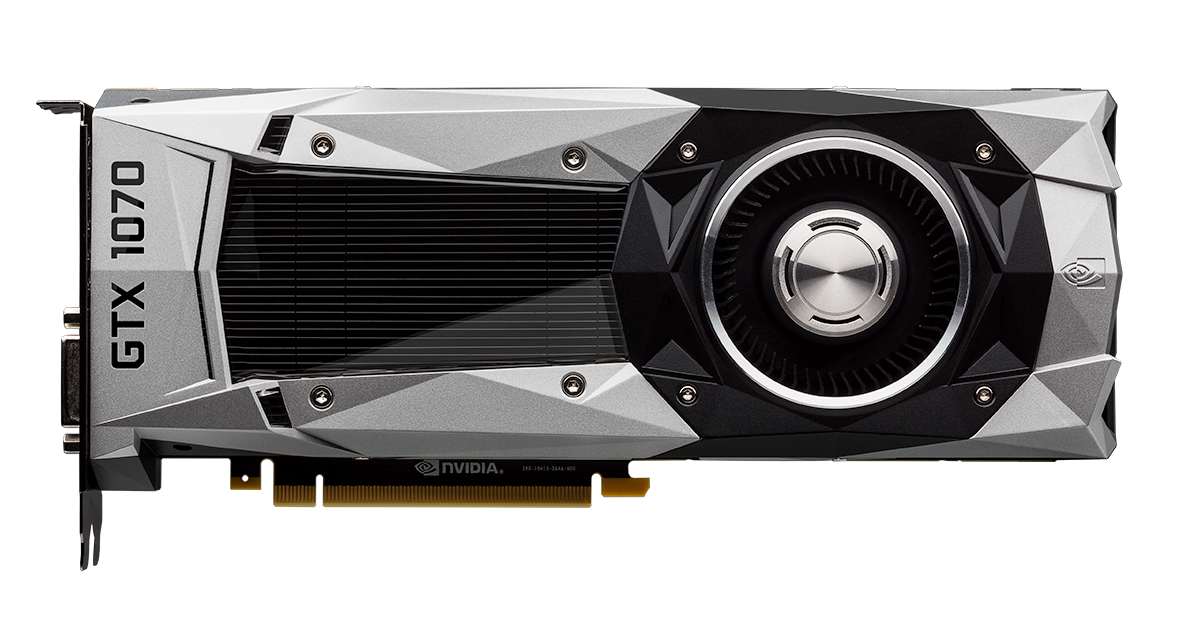
\includegraphics[width=0.7\linewidth]{images/geforce-gtx-1070-2c50-P@2x}
	\captionsetup{labelformat=empty}
	\caption{Geforce GTX 1070}
\end{figure}


\subsection*{7.2 How Does GPU Mining Work?}
GPU mining became a hot topic in 2017 after Bitcoin zapped past its previous highs to peak at just under \$20,000 (a little less than half of what it would later reach in January 2021!). Since then, individuals from around the world have sought the best GPUs to get their share of crypto block rewards.\vspace{.3 cm}

The complex maths functions solved by computers are usually SHA-256 hash functions. In mining, the computer takes the SHA-256 — an encrypted mathematical algorithm — and turn it into an output. The output is always a 256-bit number.\vspace{.3 cm}

\subsection*{7.3 The Sha-256 Hash Function}
Encrypted in the SHA-256 problems solved by computers are details of electronic payments and algorithms necessary to secure a blockchain network from attackers wishing to "double-spend." For partaking in the security of the blockchain network, miners are rewarded with crypto coins.\vspace{.3 cm}

When the computational problem is solved by the mining card, the product is a seemingly-random 64 character output called a hash. On the Bitcoin network, miners have to find a hash that starts with approximately seventeen zeroes. To get this number, a computer has to try multiple times.\vspace{.3 cm}

Once the hash is found, the block is closed, and the miner/pool of miners are rewarded with newly-created Bitcoin and transaction fees. On any blockchain, the hash rate is the speed at which a miner arrives and finds a hash. The hash rate is measured in giga hashes (GH/s).\vspace{.3 cm}

\section*{8. GPU Mining Algorithms}
\addcontentsline{toc}{chapter}{GPU Mining Algorithms}
Just as there are different cryptocurrencies built on different blockchains, there are different types of cryptocurrency mining algorithms available. The hash (the product of mining) differs on the different types of blockchain.\vspace{.3 cm}

A hashing algorithm is a cryptographic hash function that maps data of any random size to a hash of a fixed size. These mathematical functions condense data to a fixed size. Because they are smaller, it is more convenient for a computer to compute hashes and solve the problems in the files or data string.\vspace{.3 cm}

The hashing algorithms available that support GPU mining are the following.\vspace{.3 cm}

\subsection*{8.1 SHA-256 Algorithm:}
SHA-256, also known as cryptographic hash algorithm, is a cryptographic function. SHA-256 algorithms function on a 512-bit message block and a 256-bit intermediate hash value. The hash rate for the SHA-256 algorithm is measured in gigahashes (GH/s).\vspace{.3 cm}

The product of mining a SHA-256 algorithm is a 32-byte (256-bit) signature for text strings. The block time varies between 6 to 10 minutes. Bitcoin (BTC), Bitcoin Cash (BCH), Terracoin (TRC) and Peercoin (PPC) are based on the SHA-256 algorithm.\vspace{.3 cm}

\subsection*{8.2 Scrypt Algorithm:}
The Scrypt hash function is used by Litecoin (LTC) as an alternative to the more power-hungry SHA-256 algorithm. Solving the Scrypt algorithm is a lot faster than the SHA-256 algorithm. The hash rate of the Scrypt algorithm is measured in kilohashes (KH/s).\vspace{.3 cm}

Scrypt runs on password-based key functions, which were created for the Tarsnap online backup service by Colin Percival. This algorithm creates many pseudorandom numbers for storing in RAM locations, which makes it almost impossible for large-scale hardware attacks to be performed on a network.\vspace{.3 cm}

Scrypt was first implemented in cryptocurrency by an anonymous programmer called ArtForz in Tenebrix, then Fairbrix and Litecoin shortly after.\vspace{.3 cm}

The block generation time of the Scrypt function is 2.5 minutes for many cryptocurrencies. As a result, they can be performed on the GPUs of computers. Dogecoin (DOGE), Latium (LAT) and Bitmark (BTM) are some other cryptocurrencies based on the Scrypt algorithm. \vspace{.3 cm}

\subsection*{8.3 X11 Algorithm:}
This is the most energy-efficient mining algorithm for GPUs. With the X11 Algorithm, the GPUs can run on 30\% less wattage. Proof-of-work blockchains that implement this algorithm run on a sequence of eleven hashing algorithms. \vspace{.3 cm}

This algorithm was implemented in the Darkcoin protocol (later renamed to Dash) in 2014, specifically made by Evan Duffield to be resistant to ASIC mining.\vspace{.3 cm}

The hash rate of the X11 Algorithm is measured in megahashes (MH/s). Some of the cryptocurrencies that use the X11 algorithm are Dash (DASH), StartCoin (START), CannabisCoin (CANN) and XCurrency (XC).\vspace{.3 cm}

\subsection*{8.4 Ethash Algorithm:}
The most well-known cryptocurrency to implement the Ethash Algorithm is Ethereum (ETH), the crypto for which this algorithm was initially created. DaggerHashimoto was the name of the first version of the Ethash algorithm, designed by Vitalik Buterin and the Ethereum team to be ASIC-resistant.\vspace{.3 cm} 

DaggerHashimoto is a combination of two other algorithms. The first, the Dagger algorithm, was built as an alternative for memory-intensive algorithms like Scrypt. However, Dagger is susceptible to pressure in shared memory hardware acceleration. The Hashimoto algorithm was designed to attain ASIC resistance by being IO-bound.\vspace{.3 cm}

The hash rate for the DaggerHashimoto algorithm is measured in megahashes (MH/s). The popular cryptocurrencies that are based on it include Ethereum, Ethereum Classic and Expanse.\vspace{.3 cm}

\subsection*{8.5 What to Mine With GPUs}
Choosing a cryptocurrency to mine with GPUs is one of the major problems new miners face. In making the decision, one of the most frequently asked questions has been how much one can make from mining cryptocurrencies with GPUs.\vspace{.3 cm}

To start, the project must be built on a blockchain architecture that supports proof-of-work (PoW) before it can be mined with GPUs. Also, different factors affect how much rewards one can make from GPU, including the block rewards.\vspace{.3 cm}

The block reward is the amount of crypto given to a miner/pool of miners for completing a block of cryptographic equations on a blockchain. \vspace{.3 cm}

For example, when Bitcoin launched in 2009, mining one block would earn you 50 BTC. However, in 2012, the block reward was halved to 25 BTC. By 2016, this was halved again to 12.5 BTC. Finally, in May 2020, the reward halved again to 6.25 BTC.\vspace{.3 cm}

The best cryptos to mine are those that give rewards that can cover the electricity charges used in mining and the cost of the mining device/rigs.\vspace{.3 cm}

\section*{9. Best Crypto to Mine With GPU}
\addcontentsline{toc}{chapter}{ Best Crypto to Mine With GPU}
Some of the best cryptos to mine with GPU in 2021 are the following.

\subsection*{9.1 Grin (GRIN)}
Grin is a relatively new cryptocurrency with high block rewards. Although the complexity of mining changes dynamically on the Grin network, mining is relatively easy and the project offers unlimited coins — a joy for miners. 60 GRIN is rewarded per block mined. A grin coin currently trades at \$0.34 as of Feb. 1, 2021.

\subsection*{9.2 Bitcoin Gold (BTG)}
This is one of the few cryptocurrencies created specifically for GPU mining. The architecture is perfectly optimized to support GPU mining. It is also one of the few non-stablecoin cryptos that have a relatively stable price.

Bitcoin Gold implements the Zhash hashing function and offers 12.5 BTG for a mined block. A BTG currently trades at \$10.65 as of Feb. 1, 2021.

\subsection*{9.3 Litecoin (LTC)}
Litecoin was one of the first users of the Scrypt protocol, meaning the network is best suited for GPU mining. Litecoin can be mined without an ASIC because it uses the SCRYPT protocol. The network also provides high-speed transactions with low fees.

Completing a block earns you a 12.5 LTC. Litecoin is currently valued at \$132 as of Feb. 1, 2021.

\section*{10. Top Picks for the Best Mining GPUs}
\addcontentsline{toc}{chapter}{Top Picks for the Best Mining GPUs}
For those still interested, we've considered the options and come up with this list of the best mining GPUs for Ethereum right now — things can change rapidly based on pricing and availability, not to mention the valuation of Ethereum and Bitcoin.\vspace{.3cm}

\subsection*{10.1GeForce RTX 3060 Ti:} The second least expensive of the Ampere GPUs, it's just as fast as the RTX 3070 and generally costs less. After tuning, it's also the most efficient GPU for Ethereum right now, using under 120W while breaking 60MH/s. Make sure you get one of the non-LHR models, though, or mining profitability with Ethereum will be terrible.

\begin{figure}[h]
	\centering
	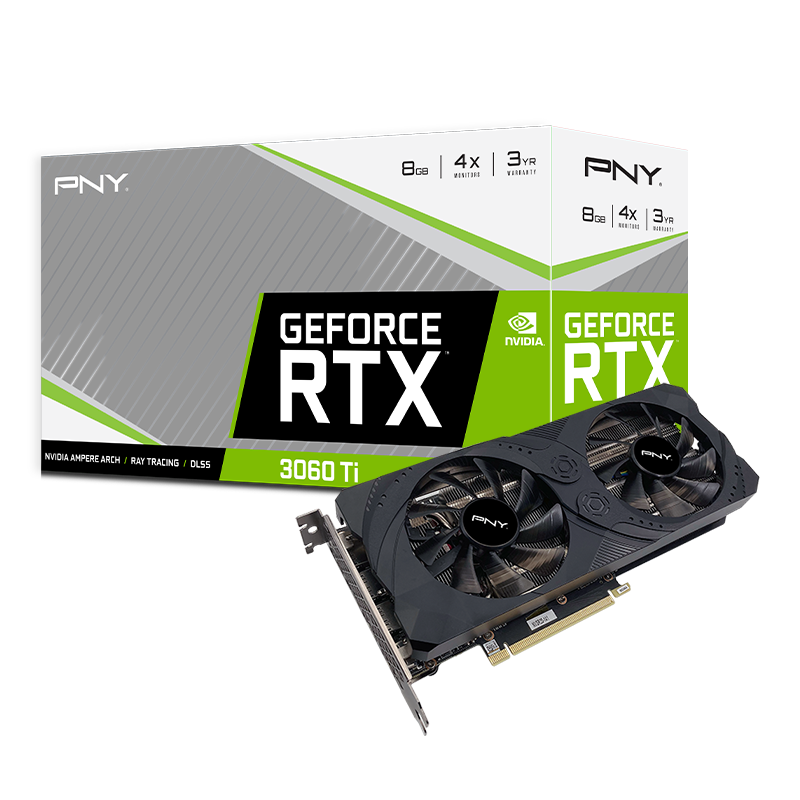
\includegraphics[width=0.5\linewidth]{7_PNY-GeForce-RTX-3060Ti-DF-M-gr}
	\captionsetup{labelformat=empty}
	\caption{RTX 3060 Ti}
\end{figure}

\subsection*{10.2 Radeon RX 5600 XT:} AMD's previous generation Navi GPUs are very good at mining, and the 5600 XT can hit about 40MH/s while using about 115W of power. The vanilla RX 5700 is another good choice, as it's as fast as the 5700 XT and costs less, but it's not as readily available.

\subsection*{10.3 GeForce RTX 2060 Super / RTX 2070:} Ethereum mining needs a lot of memory bandwidth, and all of the RTX 20-series GPUs with 8GB end up at around 44MH/s and 130W of power, meaning you should buy whichever is cheapest. That's usually the RTX 2060 Super or the older RTX 2070.

\subsection*{10.4 Radeon RX 580 8GB:} All the Polaris GPUs with 8GB of GDDR5 memory (including the RX 590, RX 580 8GB, RX 570 8GB, RX 480 8GB, and RX 470 8GB) end up with relatively similar performance, depending on how well your card's memory overclocks. The RX 590 is currently the cheapest (theoretically), but it's in limited supply, so look for any of the other Polaris 10/20 GPUs. Just don't get the 4GB models!

\subsection*{10.5 GeForce GTX 1060 6GB:} Mining performance is a bit lower than the RX 580 8GB (30MH/s), but power is well under 100W in our testing after tuning. Of course these could be five years old cards by this point, and buying a used graphics card presents some obvious risks!

\subsection*{10.6 Radeon RX Vega 56/64:} Overall performance is good, and some cards can perform much better — our reference models used for testing are more of a worst-case choice for most of the GPUs. After tuning, some Vega cards might even hit 45-50MH/s, which would put this at the top of the chart.

\subsection*{10.7 Radeon RX 6800:} Big Navi is potent when it comes to hashing, and all of the cards we've tested hit similar hash rates of around 65MH/s and 170W power use. The RX 6800 is generally cheaper than the others and used a bit less power, making it the clear winner. Plus, when you're not mining, it's a very capable gaming GPU.

\begin{figure}[h]
	\centering
	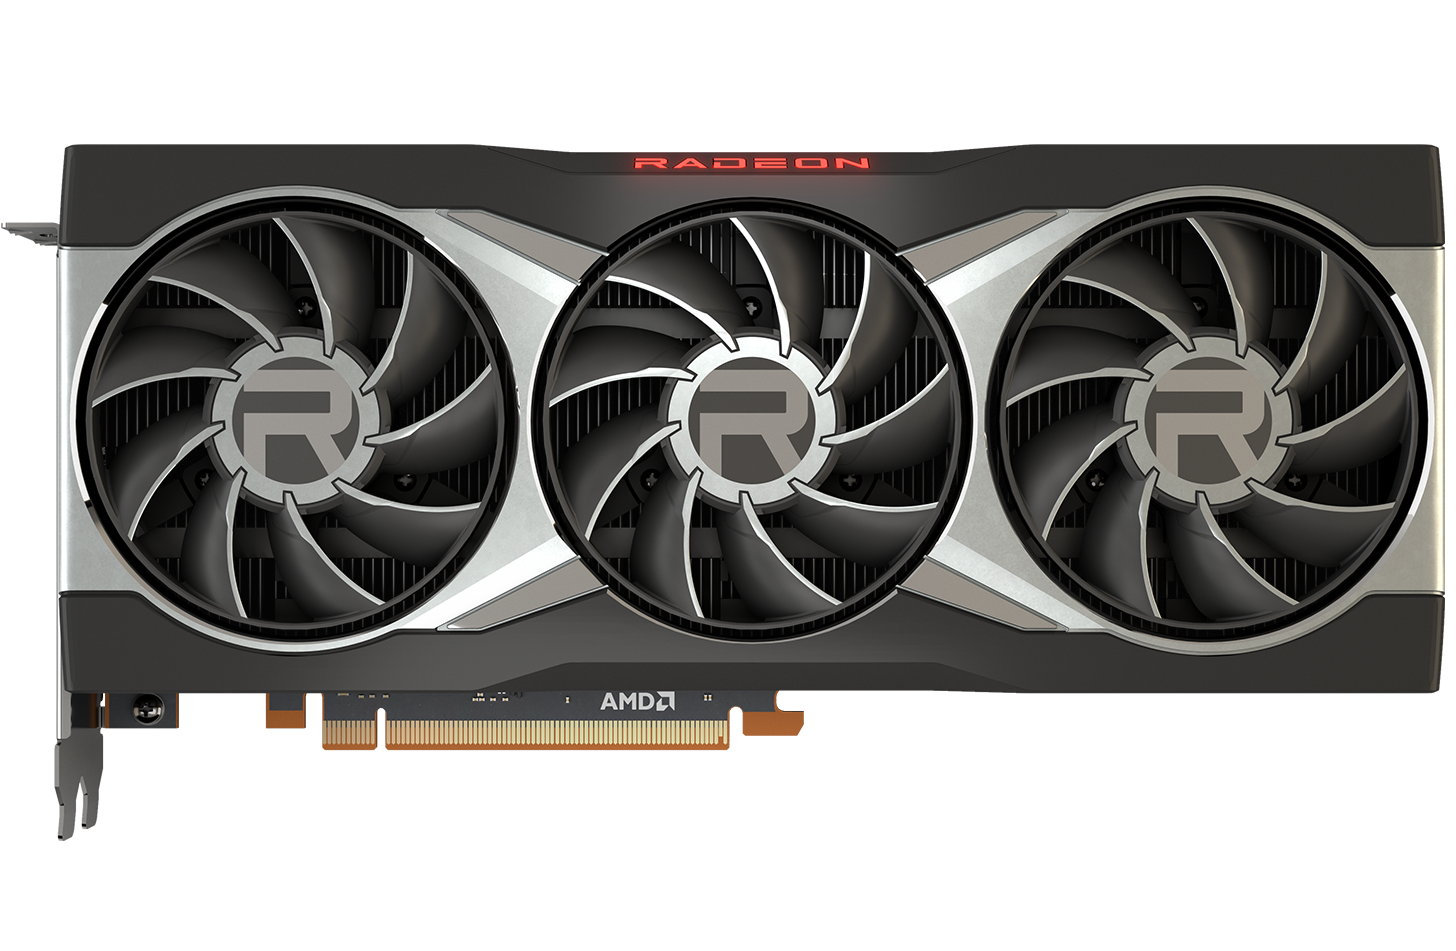
\includegraphics[width=0.7\linewidth]{kf-img}
	\captionsetup{labelformat=empty}
	\caption{Radeon RX 6800}
\end{figure}

\subsection*{10.8 GeForce RTX 3090:} This is the fastest graphics card right now, for mining and gaming purposes, and it's the only Nvidia Ampere GPU that won't be replaced by an LHR equivalent. The time to break even is pretty terrible right now, at more than a year, but if you do get into the black it will end up with the highest profitability from that point forward. But really, you shouldn't buy a \$2,500 GPU for mining right now when it only makes about \$6.50 per day.

\begin{figure}[h]
	\centering
	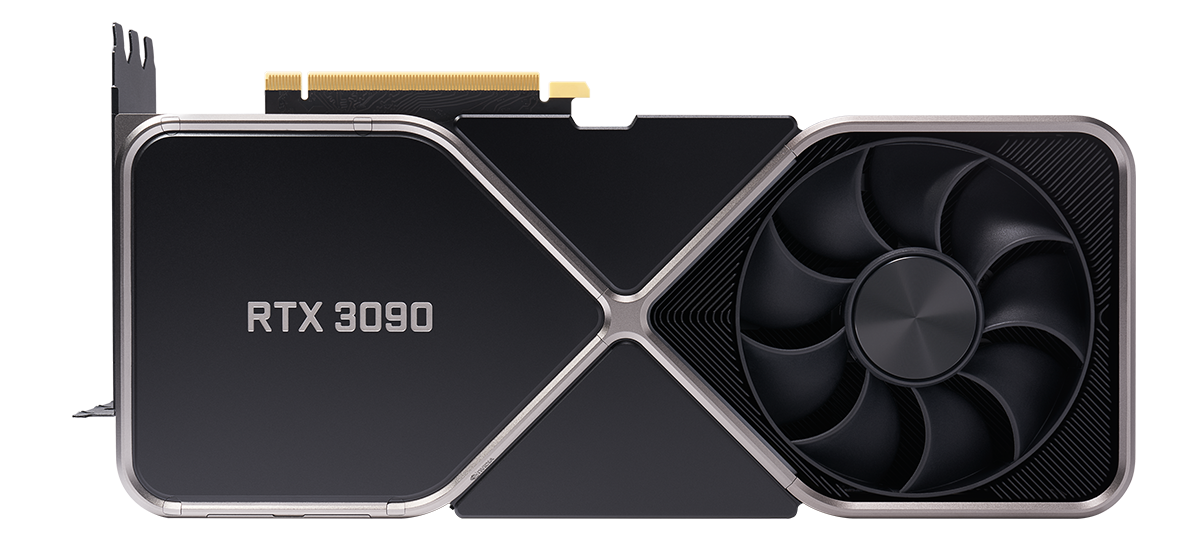
\includegraphics[width=0.7\linewidth]{images/geforce_rtx_3090_fe}
	\captionsetup{labelformat=empty}
	\caption{GeForce RTX 3090}
\end{figure}
